
\documentclass{beamer}
\usepackage{natbib}

\title{Measuring Income Tax Evasion Using Bank Credit: Evidence from Greece Get access Arrow by \citet{artavanis2016measuring}}
\author{}
\date{\today}
\begin{document}

\frame{\titlepage}

\begin{frame}
\frametitle{Some Odd Patterns in Bank Loans}
\begin{figure}
    \centering
    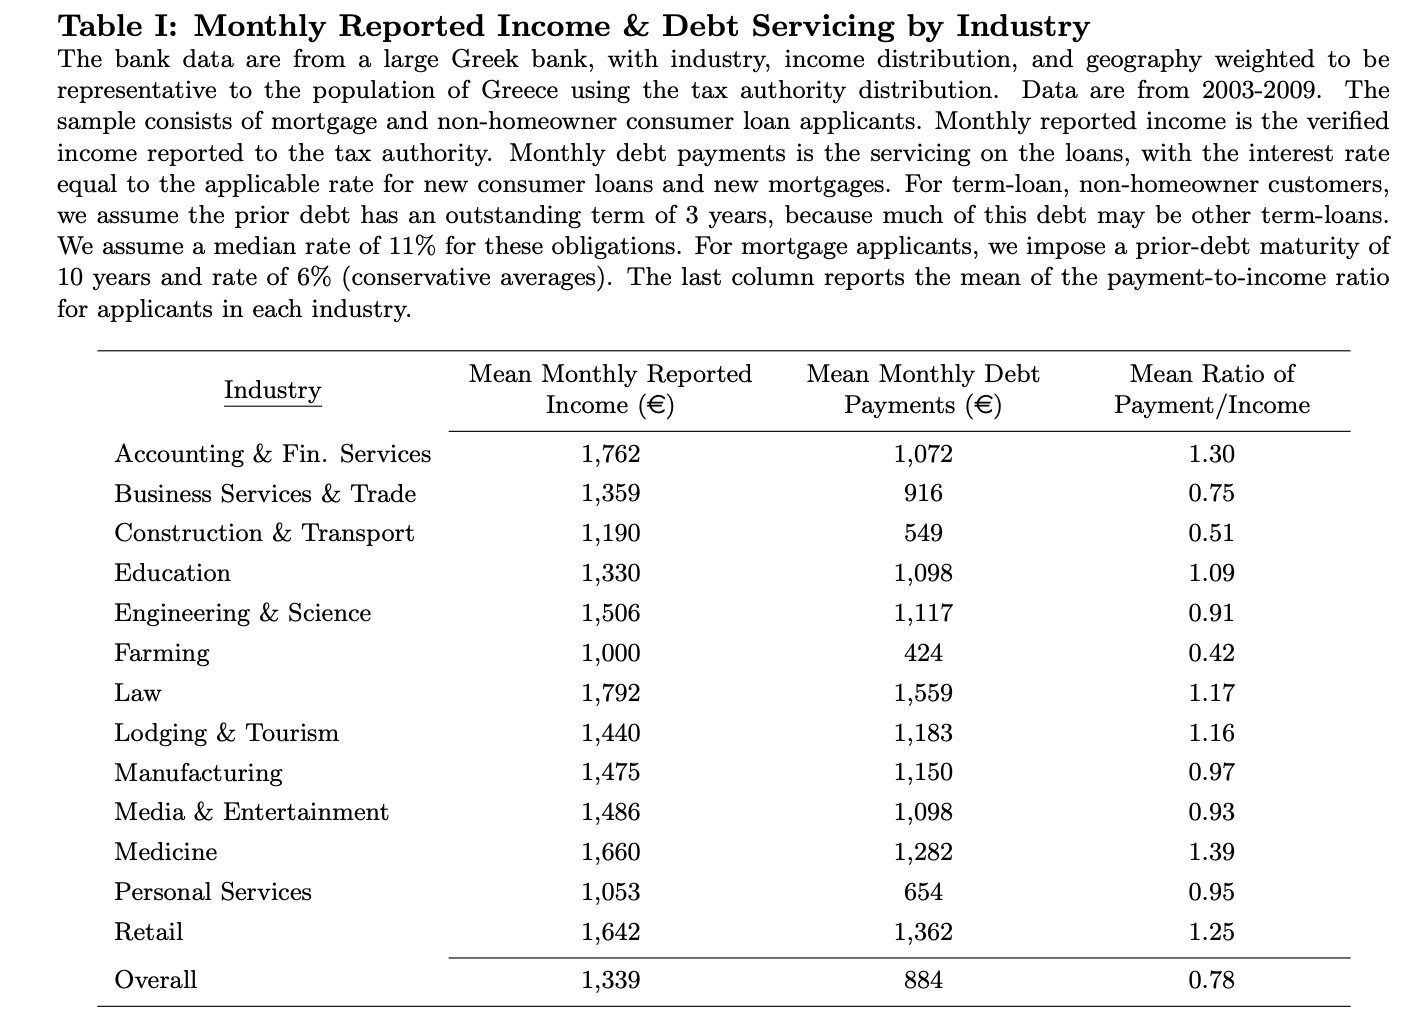
\includegraphics[width=\textwidth]{Paper Presentations/Table1.png}
\end{figure}
\end{frame}


\begin{frame}
\frametitle{Context }
\begin{itemize}
    \item Use loan decisions data from a big Greek Bank.
    \item After algorithm assigns the scores, bank managers make decisions after considering soft information such as potential real income.
    \item Data is universe of credit applications including those rejected.
    \item Tax data includes total income reported and total no of households at postal code and occupation level.
    \item Occupations: self-employed, wage workers,merchants and agriculture
    
\end{itemize}
\end{frame}

\begin{frame}{Methods}
\begin{itemize}
    \item Banks decide level of credit as a linear combination of their assessed true income, risk level and other area X individual soft skills.
    \[credit=\beta_1 Y^{True}+\Phi Risk+\Psi
    SOFT\]
    \item In data, you observe reported income $Y^R$. They use $credit$ to infer $Y^{True}$.
    \item Assume that 
    \[Y_{ij}^{True}= \begin{cases}
			\lambda_j Y_{ij}^{R}, & \text{if self-employed}\\
            Y_{ij}^R, & \text{if wage worker}
		 \end{cases}\]
   \item Use this to break credit equation to 
   \[credit_{ij}=\beta_{1j}Y^R{ij}(1-SE_i)+\beta_{2j}Y^R SE_i+f.e^{CreditGrade}+SOFT_{ij}\Psi
   \]
   $\lambda$ is ratio of the two betas. What are identifying assumptions of this equation?
\end{itemize}
\end{frame}

\begin{frame}{Results}
    \begin{figure}
        \centering
                \caption{Debt Capacity}
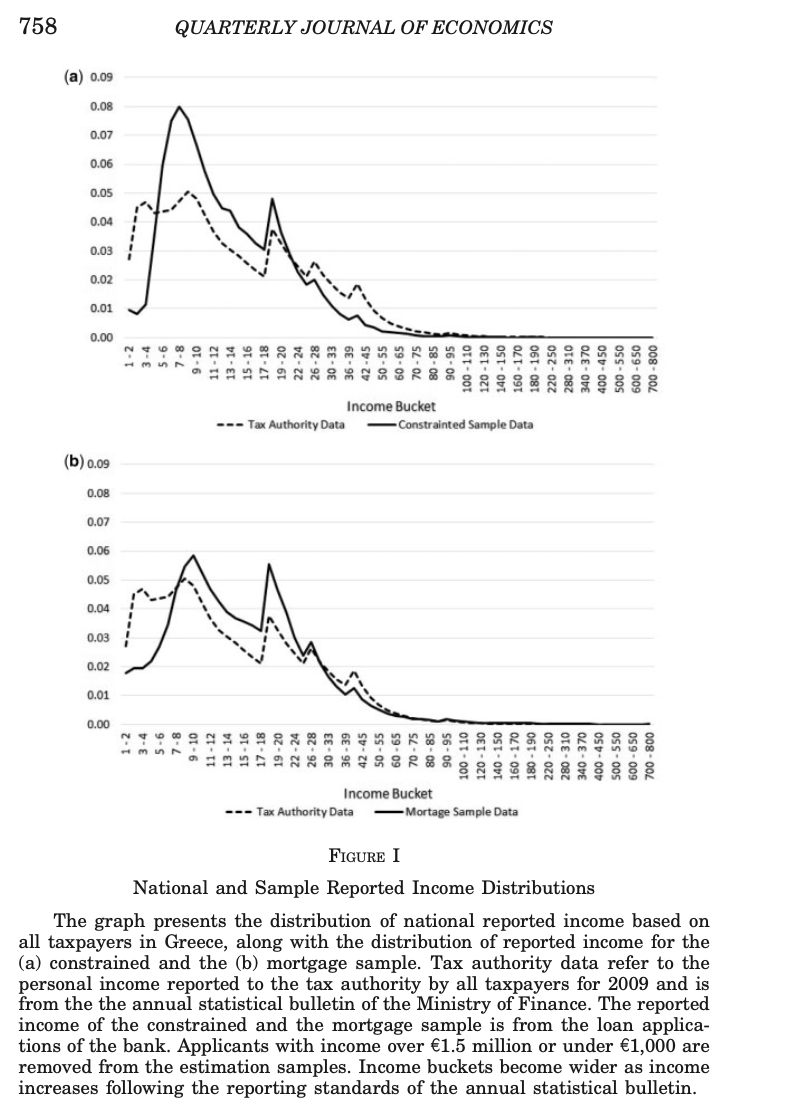
\includegraphics[height=\textheight,keepaspectratio]{Paper Presentations/R1.png}
    \end{figure}
\end{frame}

\begin{frame}{Results}
    \begin{figure}
        \centering
                \caption{Estimates}
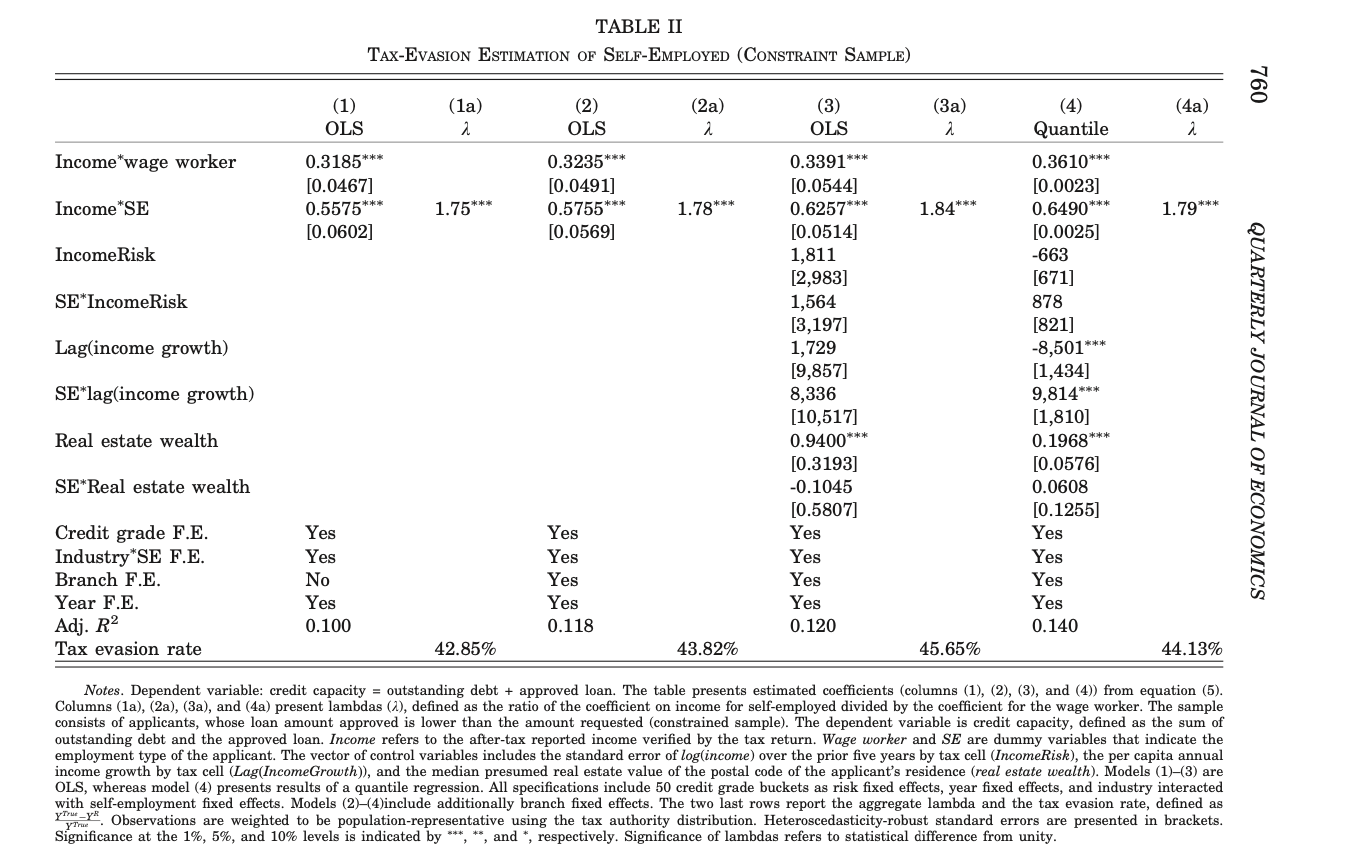
\includegraphics[width=\textwidth,height=\textheight,keepaspectratio]{Paper Presentations/T2.png}
    \end{figure}
\end{frame}

\begin{frame}{Results}
    \begin{figure}
        \centering
                \caption{Mortgage Sample}
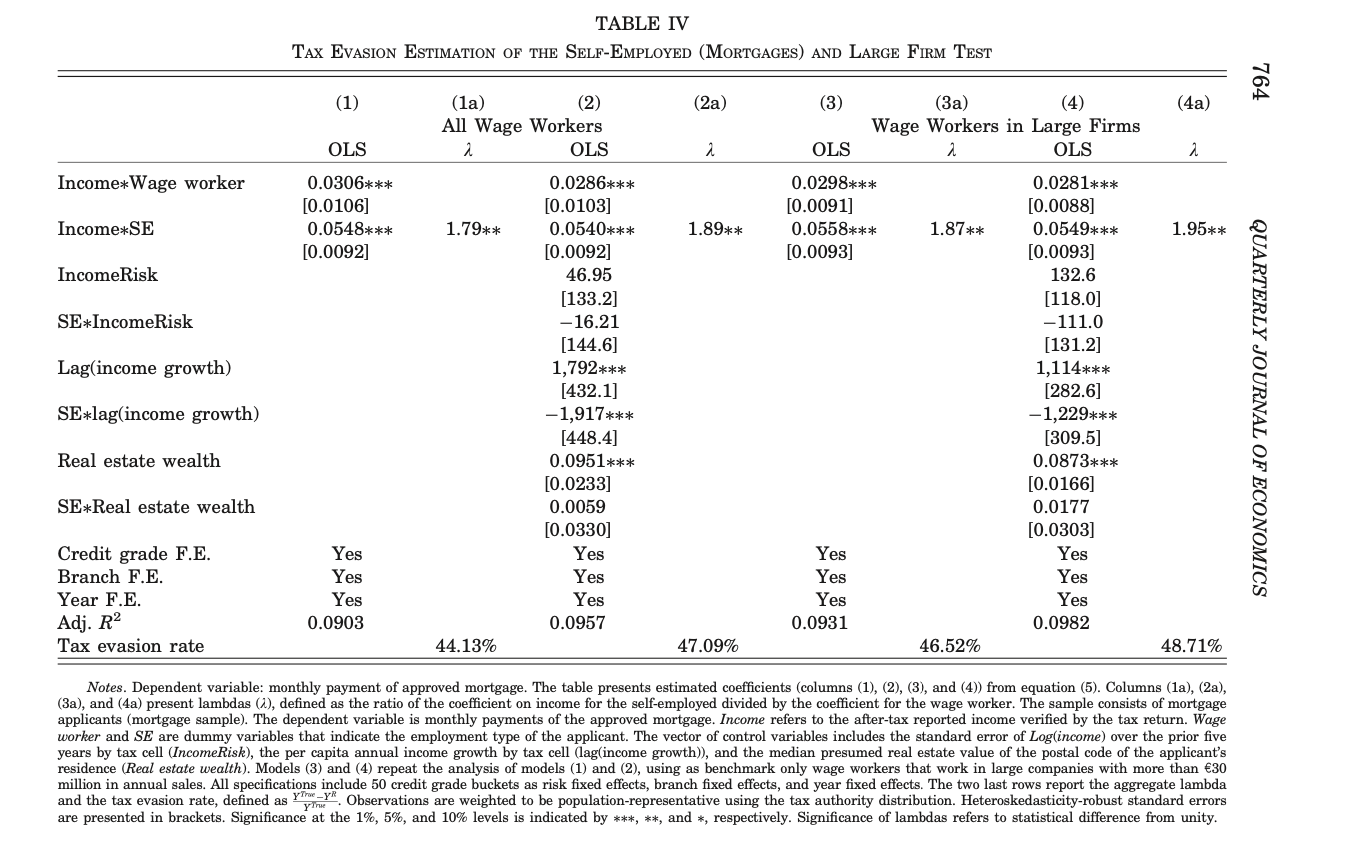
\includegraphics[width=\textwidth,height=\textheight,keepaspectratio]{Paper Presentations/T4.png}
    \end{figure}
\end{frame}

\begin{frame}
\frametitle{Results}
\begin{itemize}
    \item A $\lambda$ of 1.75 translates into 43\% evasion rate.
\end{itemize}
\end{frame}

\begin{frame}
\frametitle{Robustness}
    \begin{figure}
        \centering
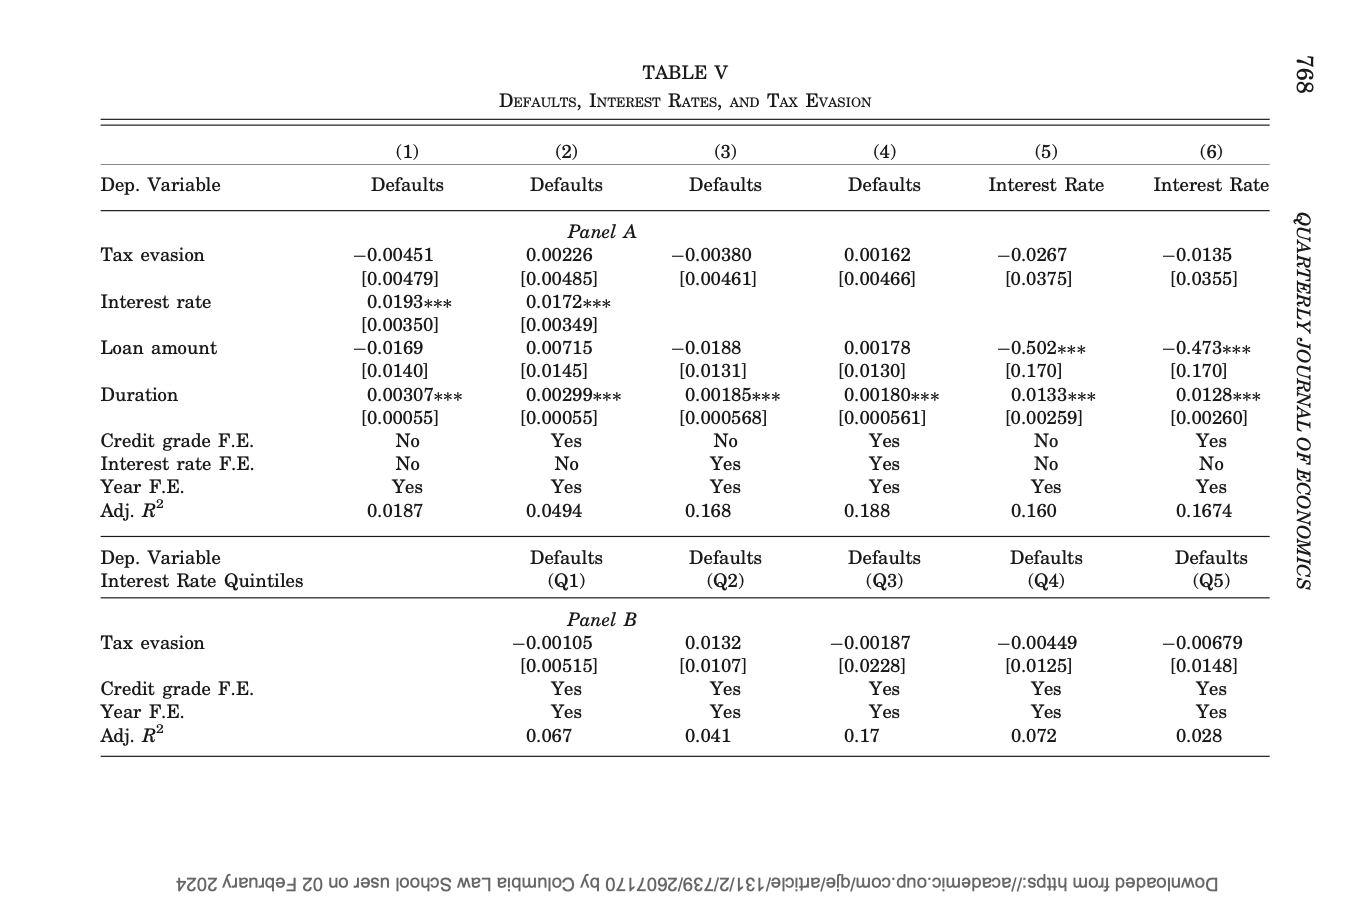
\includegraphics[width=\textwidth,height=\textheight,keepaspectratio]{Paper Presentations/T5.png}
    \end{figure}
\end{frame}

\begin{frame}
\frametitle{Evasion by Industry}
    \begin{figure}
        \centering
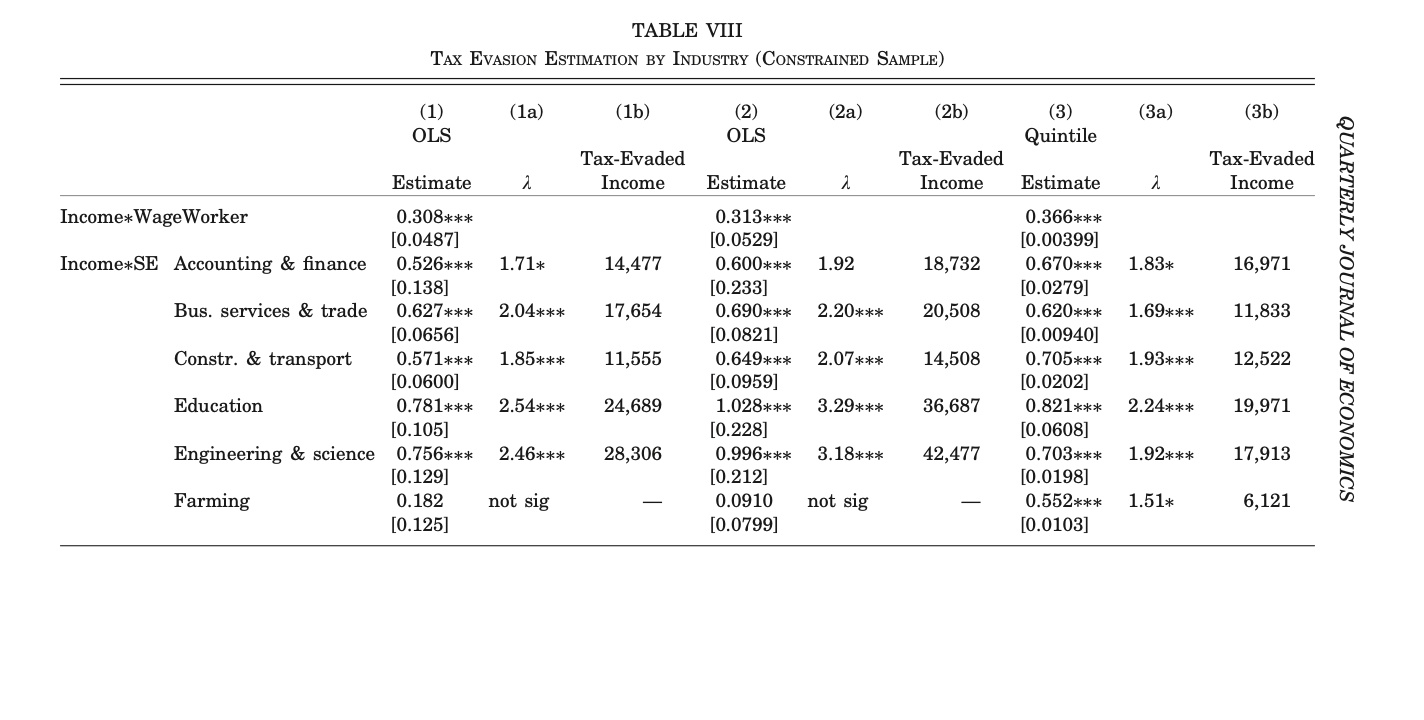
\includegraphics[width=\textwidth,height=\textheight,keepaspectratio]{Paper Presentations/T81.png}
    \end{figure}
\end{frame}
\begin{frame}
\frametitle{Evasion by Industry}
    \begin{figure}
        \centering
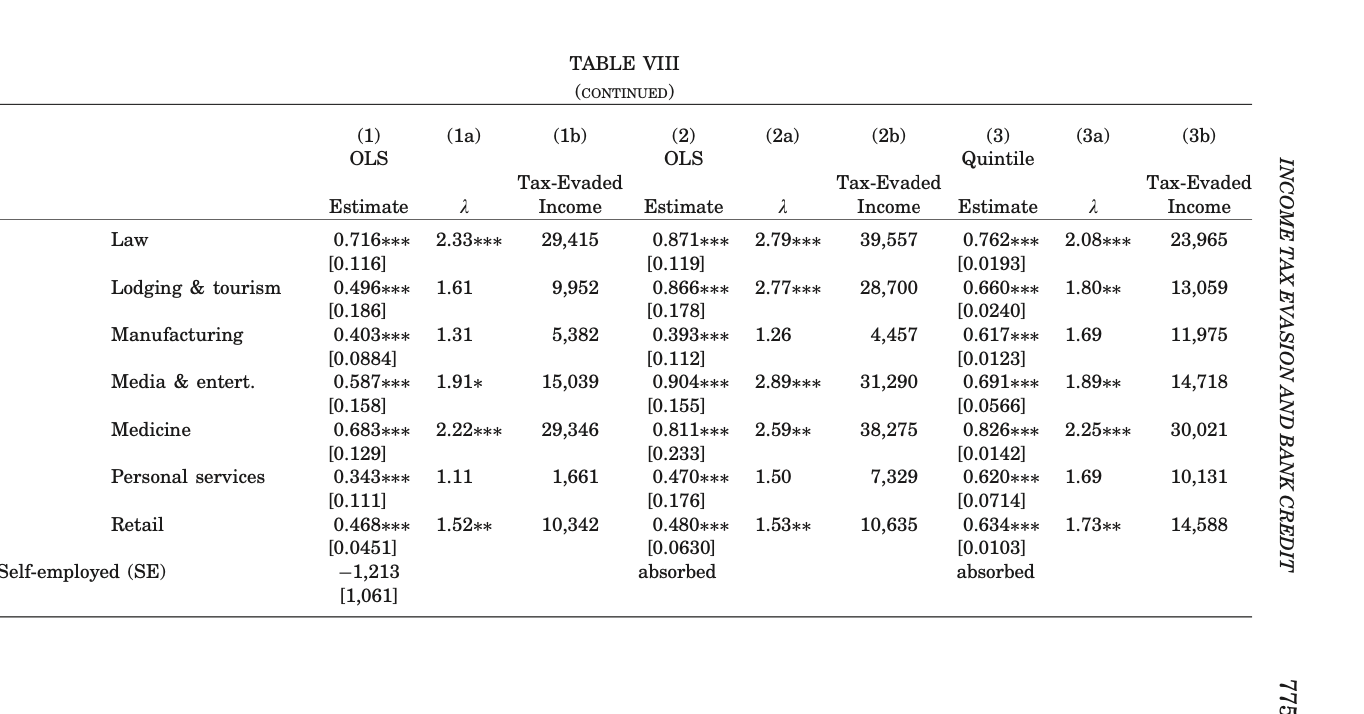
\includegraphics[width=\textwidth,height=\textheight,keepaspectratio]{Paper Presentations/T82.png}
    \end{figure}
\end{frame}

\begin{frame}
\frametitle{Robustness: Paper Trail}
    \begin{figure}
        \centering
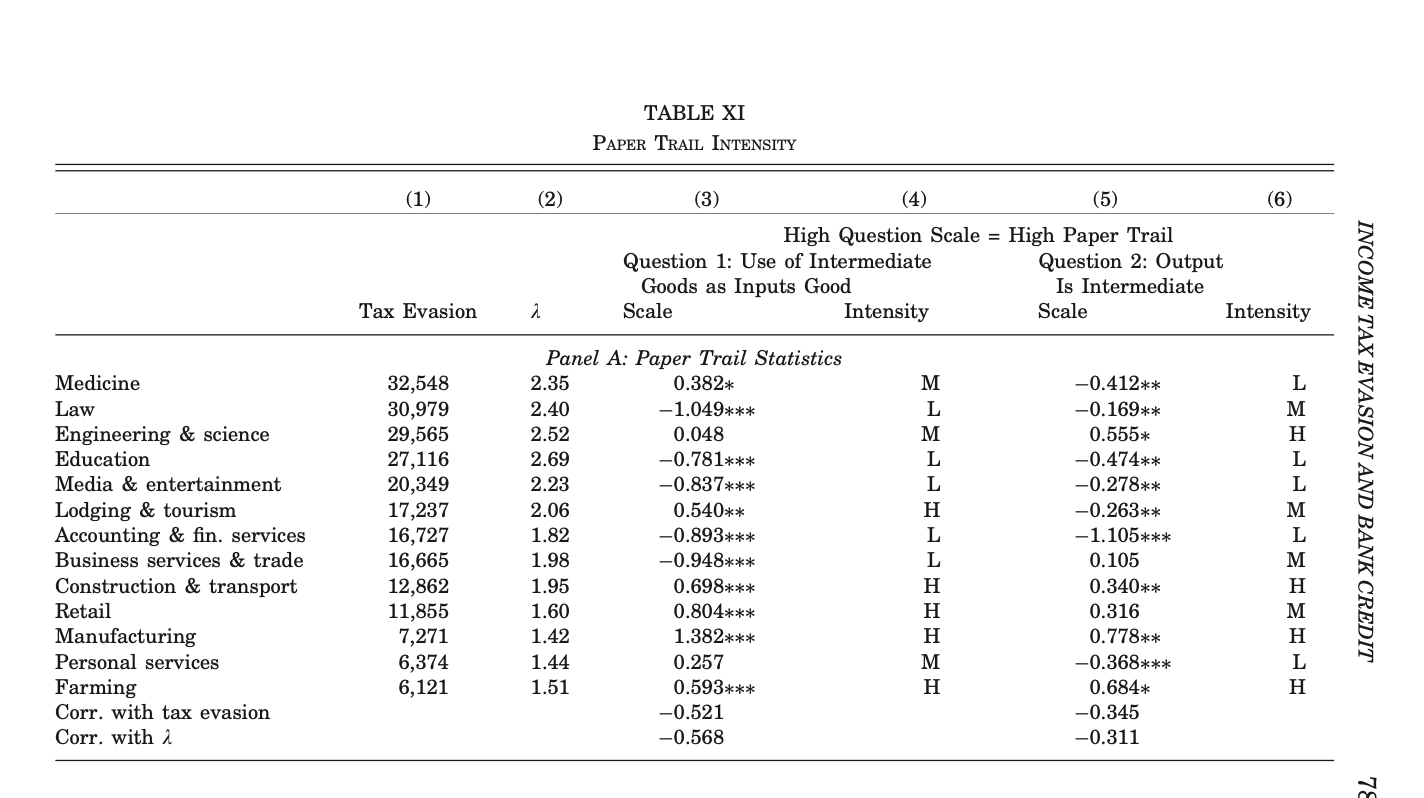
\includegraphics[width=\textwidth,height=\textheight,keepaspectratio]{Paper Presentations/T9.png}
    \end{figure}
\end{frame}

\begin{frame}
\frametitle{Robustness: Paper Trail}
    \begin{figure}
        \centering
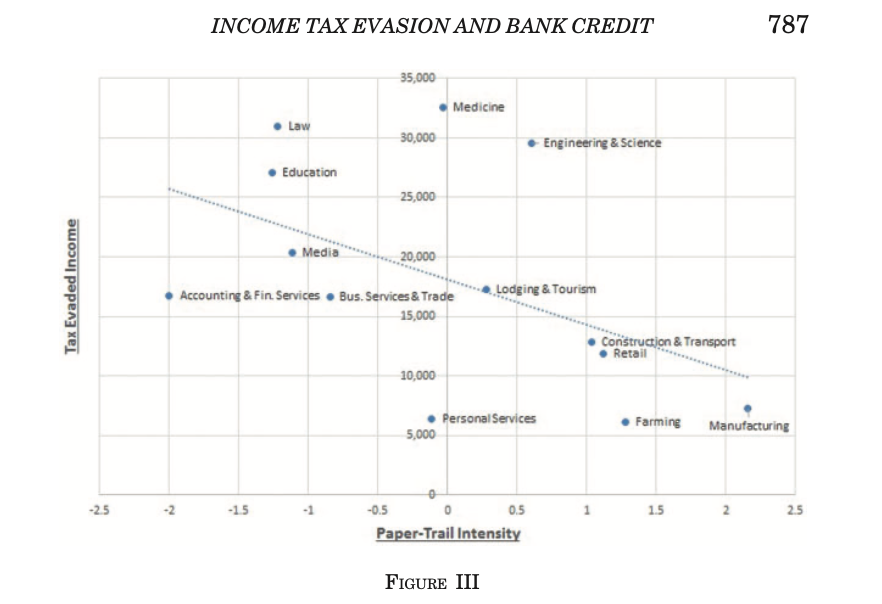
\includegraphics[width=\textwidth,height=\textheight,keepaspectratio]{Paper Presentations/F2.png}
    \end{figure}
\end{frame}

\begin{frame}
\frametitle{Mechanism}
    \begin{figure}
        \centering
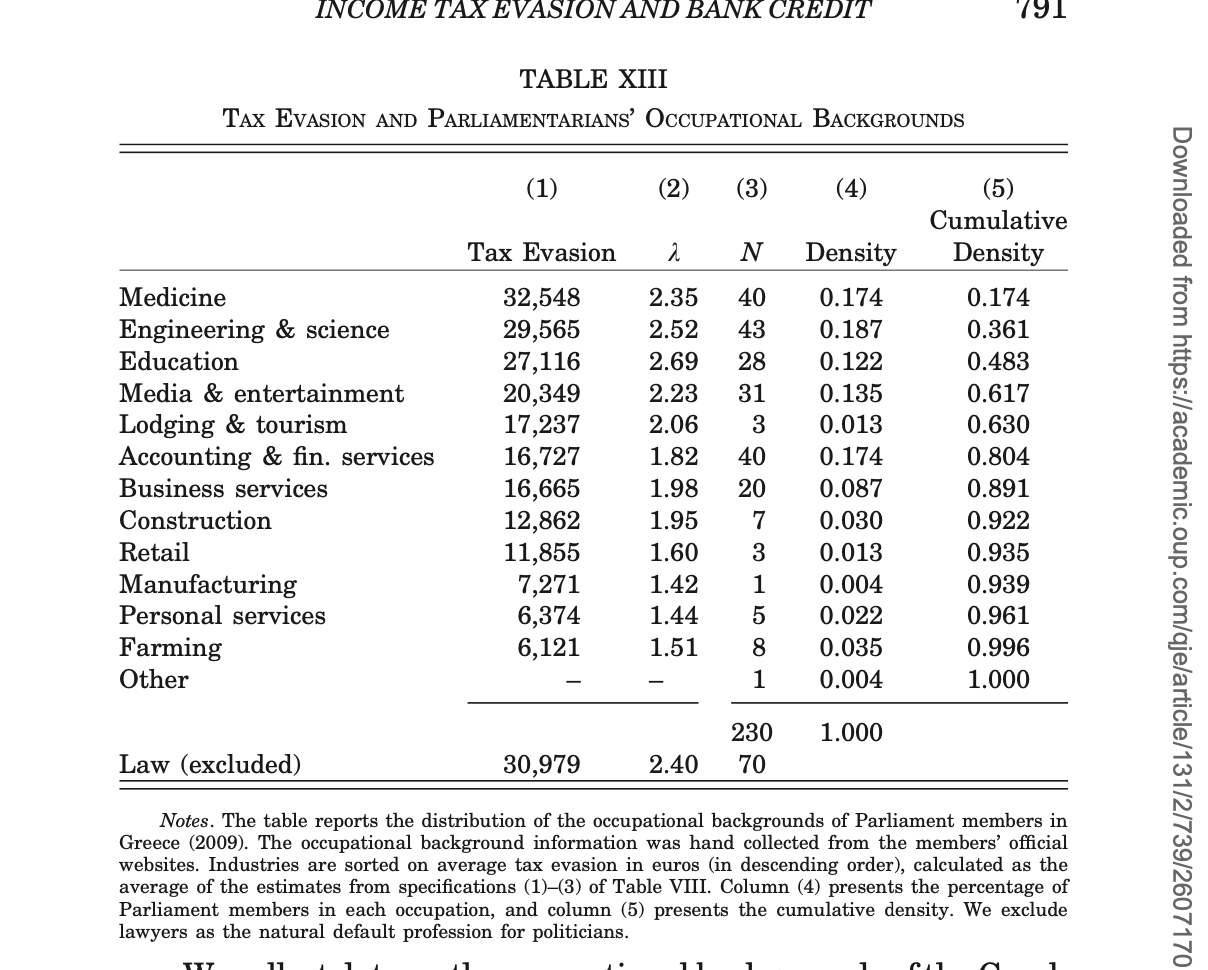
\includegraphics[width=\textwidth,height=\textheight,keepaspectratio]{Paper Presentations/T13.png}
    \end{figure}
\end{frame}

\begin{frame}{Discussion}
\begin{quote}
    How does our 43–45\% estimated tax evasion rate compare with previous studies? Pissarides and Weber (1989) find that on average, the true income of self-employed individuals in Great Britain is 1.55 times their reported income, which corresponds to a tax evasion rate of 35\%. Kleven et al. (2011) show underre- porting of 41.6\% in Denmark for self-employed income, while re- search building off the Tax Compliance Measurement Program (Slemrod 2007; Black et al. 2012) estimate an underreporting for the United States of approximately 50\% for the self-employed. Galbiati and Zanella (2012) report an evasion rate of 46.6\% for Italy, whereas Braguinsky, Mityakov, and Liscovich (2014) find 80\% tax evasion rates in Russia.
\end{quote}
    
\end{frame}
\end{document}
